% !TEX TS-program = xelatex
% !TeX spellcheck = ru_RU
% !TEX root = talk.tex

\documentclass
  [ russian
  , aspectratio=1610
  ] {beamer}

% !TeX spellcheck = ru_RU
% !TEX root = talk.tex
% Опциональные добавления используемых пакетов. Вполне может быть, что они вам не понадобятся, но в шаблоне приведены примеры их использования.
\usepackage{tikz} % Мощный пакет для создание рисунков, однако может очень сильно замедлять компиляцию
\usetikzlibrary{decorations.pathreplacing,calc,shapes,positioning,tikzmark}

% Библиотека для TikZ, которая генерирует отдельные файлы для каждого рисунка
% Позволяет ускорить компиляцию, однако имеет свои ограничения
% Например, ломает пример выделения кода в листинге из шаблона
% \usetikzlibrary{external}
% \tikzexternalize[prefix=figures/]

\newcounter{tmkcount}

\tikzset{
    use tikzmark/.style={
            remember picture,
            overlay,
            execute at end picture={
                    \stepcounter{tmkcount}
                },
        },
    tikzmark suffix={-\thetmkcount}
}

\usepackage{booktabs} % Пакет для верстки "более книжных" таблиц, вполне годится для оформления результатов
% В шаблоне есть команда \multirowcell, которой нужен этот пакет.
\usepackage{multirow}
\usepackage{siunitx} % для таблиц с единицами измерений

% Для названий стоит использовать \textsc{}
\newcommand{\OCaml}{\textsc{OCaml}}
\newcommand{\miniKanren}{\textsc{miniKanren}}
\newcommand{\BibTeX}{\textsc{BibTeX}}
\newcommand{\vsharp}{\textsc{V$\sharp$}}
\newcommand{\fsharp}{\textsc{F$\sharp$}}
\newcommand{\csharp}{\textsc{C\#}}
\newcommand{\GitHub}{\textsc{GitHub}}
\newcommand{\SMT}{\textsc{SMT}}

\definecolor{eclipseGreen}{RGB}{63,127,95}
% \lstdefinelanguage{ocaml}{
% keywords={@type, function, fun, let, in, match, with, when, class, type,
% nonrec, object, method, of, rec, repeat, until, while, not, do, done, as, val, inherit, and,
% new, module, sig, deriving, datatype, struct, if, then, else, open, private, virtual, include, success, failure,
% lazy, assert, true, false, end},
% sensitive=true,
% commentstyle=\small\itshape\ttfamily,
% keywordstyle=\ttfamily\bfseries, %\underbar,
% identifierstyle=\ttfamily,
% basewidth={0.5em,0.5em},
% columns=fixed,
% fontadjust=true,
% literate={->}{{$\to$}}3 {===}{{$\equiv$}}1 {=/=}{{$\not\equiv$}}1 {|>}{{$\triangleright$}}3 {\\/}{{$\vee$}}2 {/\\}{{$\wedge$}}2 {>=}{{$\ge$}}1 {<=}{{$\le$}} 1,
% morecomment=[s]{(*}{*)}
% }

\makeatletter
\@ifclassloaded{beamer}{
    %%% Обязательные пакеты
    %% Beamer
    \usepackage{beamerthemesplit}
    \usetheme{SPbGU}
    \beamertemplatenavigationsymbolsempty
    \usepackage{appendixnumberbeamer}

    %% Локализация
    \usepackage{fontspec}
    \setmainfont{CMU Serif}
    \setsansfont{CMU Sans Serif}
    \setmonofont{CMU Typewriter Text}
    %\setmonofont{Fira Code}[Contextuals=Alternate,Scale=0.9]
    %\setmonofont{Inconsolata}
    \usepackage{polyglossia}
    \setmainlanguage{russian}
    \setotherlanguage{english}

    %% Графика
    \usepackage{pdfpages} % Позволяет вставлять многостраничные pdf документы в текст

    % Математические окружения с русским названием
    \newtheorem{rutheorem}{Теорема}
    \newtheorem{ruproof}{Доказательство}
    \newtheorem{rudefinition}{Определение}
    \newtheorem{rulemma}{Лемма}
    \usepackage{fancyvrb}
}
{}
\makeatother

\usepackage[autostyle]{csquotes} % Правильные кавычки в зависимости от языка
\usepackage{totcount}
\usepackage{setspace}
\usepackage{amsmath, amsfonts, amssymb, amsthm, mathtools} % "Адекватная" работа с математикой в LaTeX


\makeatletter

%!TEX root = talk.tex

%% Параметры заполнения титульного листа
\usepackage{xkeyval}

%% Русскоязычный вариант
\define@key[ru]{mytitle}{chair}{\def\my@title@chair@ru{#1}}
\define@key[ru]{mytitle}{title}{\def\my@title@title@ru{#1}}
\define@key[ru]{mytitle}{group}{\def\my@title@group@ru{#1}}
\define@key[ru]{mytitle}{author}{\def\my@title@author@ru{#1}}
\define@key[ru]{mytitle}{supervisor}{\def\my@title@supervisor@ru{#1}}
\define@key[ru]{mytitle}{supervisorPosition}{\def\my@title@supervisorPosition@ru{#1}}
\define@key[ru]{mytitle}{reviewer}{\def\my@title@reviewer@ru{#1}}
\define@key[ru]{mytitle}{reviewerPosition}{\def\my@title@reviewerPosition@ru{#1}}
\define@key[ru]{mytitle}{consultant}{\def\my@title@consultant@ru{#1}}
\define@key[ru]{mytitle}{consultantPosition}{\def\my@title@consultantPosition@ru{#1}}
\define@key[ru]{mytitle}{year}{\def\my@title@year@ru{#1}}
\define@key[ru]{mytitle}{specialty}{\def\my@title@specialty@ru{#1}}
\define@key[ru]{mytitle}{programme}{\def\my@title@programme@ru{#1}}
\define@key[ru]{mytitle}{profile}{\def\my@title@profile@ru{#1}}
\define@choicekey*[ru]{mytitle}{type}{coursework,practice,prediploma,master,bachelor,production}{\def\my@title@type@ru{#1}}
\define@choicekey*[ru]{mytitle}{kind}{solution,experiment,production,comparison,theoretical}{\def\my@title@kind@ru{#1}}

%% Англоязычный вариант
\define@key[en]{mytitle}{chair}{\def\my@title@chair@en{#1}}
\define@key[en]{mytitle}{title}{\def\my@title@title@en{#1}}
\define@key[en]{mytitle}{group}{\def\my@title@group@en{#1}}
\define@key[en]{mytitle}{author}{\def\my@title@author@en{#1}}
\define@key[en]{mytitle}{supervisor}{\def\my@title@supervisor@en{#1}}
\define@key[en]{mytitle}{supervisorPosition}{\def\my@title@supervisorPosition@en{#1}}
\define@key[en]{mytitle}{reviewer}{\def\my@title@reviewer@en{#1}}
\define@key[en]{mytitle}{reviewerPosition}{\def\my@title@reviewerPosition@en{#1}}
\define@key[en]{mytitle}{consultant}{\def\my@title@consultant@en{#1}}
\define@key[en]{mytitle}{consultantPosition}{\def\my@title@consultantPosition@en{#1}}
\define@key[en]{mytitle}{year}{\def\my@title@year@en{#1}}
\define@key[en]{mytitle}{specialty}{\def\my@title@specialty@en{#1}}
\define@key[en]{mytitle}{programme}{\def\my@title@programme@en{#1}}
\define@key[en]{mytitle}{profile}{\def\my@title@profile@en{#1}}
\define@choicekey*[en]{mytitle}{type}{coursework,practice,prediploma,master,bachelor}{\def\my@title@type@en{#1}}
\define@choicekey*[en]{mytitle}{kind}{solution,experiment,production,comparison,theoretical}{\def\my@title@kind@en{#1}}

\newcommand{\filltitle}[2]{
    %% Значения по умолчанию для обоих языков
    \ifthenelse{\equal{#1}{ru}}
    {
        \presetkeys[#1]{mytitle}{
            year = {\the\year},
            type = {practice},
            reviewer = {},
            consultant = {},
            profile = {}
        }{}
    }
    {}
    \ifthenelse{\equal{#1}{en}}
    {
        \presetkeys[#1]{mytitle}{
            year = {\the\year},
            type = {practice},
            reviewer = {},
            consultant = {},
            profile = {}
        }{}
    }
    {}
    \setkeys[#1]{mytitle}{#2}
}


% !TeX spellcheck = ru_RU
% !TEX root = talk.tex

%% Если что-то забыли, при компиляции будут ошибки Undefined control sequence \my@title@<что забыли>@ru
\filltitle{ru}{
    chair              = {Кафедра системного программирования},
    group              = {23.Б11-мм},
    %
    title              = {Масштабируемость распределённого Galois на задачах анализа графов},
    %
    type               = {practice},
    %
    kind               = {experiment},
    %
    author             = {Комбаев Ильхом},
    %
    specialty          = {},
    %
    programme          = {},
    %
    supervisorPosition = {},
    supervisor         = {},
}


\newcommand{\academicGroup}{\my@title@group@ru}
\newcommand{\advisorChair}{\my@title@chair@ru}
\title[Масштабируемость D-Galois]{\my@title@title@ru}
\author[\my@title@author@ru]{\my@title@author@ru, группа \academicGroup}
\institute[СПбГУ]{}
\date[2026]{}
\newcommand{\defenseYear}{\my@title@year@ru}

\makeatother

% Подпись под рисунком
\newcommand{\figcap}[1]{\par\vspace{-2pt}{\scriptsize\itshape #1\par}\vspace{4pt}}

\begin{document}
{
\setbeamertemplate{footline}{}

\begin{frame}
    \vspace{15pt}
    \begin{center}
        \begin{tabular}{c}
            \scriptsize{Санкт-Петербургский государственный университет} \\
            \scriptsize{\advisorChair}
        \end{tabular}
        \titlepage
    \end{center}

    \btVFill

    \begin{center}
        \vspace{5pt}
        \scriptsize{Санкт-Петербург\\ \defenseYear}
    \end{center}
\end{frame}
}

\begin{frame}
    \frametitle{Постановка задачи}
    \textbf{Цель}: оценить сильную масштабируемость распределённого Galois (D-Galois)
    по числу процессов и объяснить, от чего она зависит
    \vspace{1em}

    \textbf{Задачи}:
    \begin{itemize}
        \item Собрать воспроизводимый стенд: Galois, графы, скрипты запуска и обработки
        \item Измерить BFS, SSSP, PageRank и подсчёт треугольников (TC) при $P = 1\ldots6$
              процессах на графах разной структуры
        \item Разложить время раунда по фазам (свой профилировщик) и объяснить результат
    \end{itemize}

    \vspace{1em}
    {\small \textbf{Сильная масштабируемость}: граф фиксирован, растёт число процессов $P$.
    ускорение $S(P) = T(1)/T(P)$, идеал $S(P) = P$}
\end{frame}

\begin{frame}
    \frametitle{Как считает D-Galois}
    \begin{columns}[T]
        \begin{column}{.5\textwidth}
            \textbf{Разбиение OEC}: каждый процесс получает непрерывный блок номеров вершин
            (\emph{мастера}) со всеми их исходящими рёбрами. Блоки подбираются так, чтобы рёбер
            было поровну

            \medskip
            Конец ребра на чужом процессе~--- \emph{зеркало}, локальная копия чужой вершины

            \medskip
            \textbf{RF} (replication factor)~--- среднее число копий вершины по всем процессам
        \end{column}
        \begin{column}{.5\textwidth}
            \textbf{Раунд} в режиме BSP (\texttt{--exec=Sync}):
            \begin{enumerate}
                \item счёт: процесс проходит своих мастеров
                \item sync: зеркала отправляют изменения мастерам
                \item Allreduce: осталась ли работа у кого-нибудь
            \end{enumerate}

            \medskip
            Следующий раунд начинается, когда все процессы закончили предыдущий
        \end{column}
    \end{columns}
\end{frame}

\begin{frame}
    \frametitle{Стенд и методика}
    \begin{columns}[T]
        \begin{column}{.45\textwidth}
            \textbf{Оборудование}
            \begin{itemize}
                \item AMD Ryzen 5 5600X: 6 ядер, общий L3 32~МБ
                \item 32~ГБ DDR4, Fedora 42
                \item GCC 15.2, Open MPI 5.0.8
                \item Galois, коммит \texttt{b67f942}
            \end{itemize}
        \end{column}
        \begin{column}{.55\textwidth}
            \textbf{Методика}
            \begin{itemize}
                \item $P$ MPI-процессов по 1 потоку, каждый на своём ядре
                \item Режим \texttt{--exec=Sync}, разбиение OEC
                \item Время~--- таймер \texttt{Timer\_N} вокруг основного цикла алгоритма,
                      без чтения и разбиения графа, максимум по процессам
                \item Медиана 5 прогонов (TC~--- 20),
                      разброс $(\max - \min)/\text{медиана} < 1\%$
            \end{itemize}
        \end{column}
    \end{columns}

    \vspace{1em}
    \textbf{Ограничение}: кластера нет, все процессы на одной машине~--- обмен идёт
    через общую память
\end{frame}

\begin{frame}
    \frametitle{Графы}
    \begin{center}
        \small
        \begin{tabular}{lrrrrr}
            \toprule
            Граф & Вершин & Рёбер & Степень: ср. / макс. & Раундов BFS & RF при $P{=}6$ \\
            \midrule
            soc-LiveJournal1  & 4.8~М & 69.0~М & 14 / 20\,293 & 16  & 3.05 \\
            roadNet-PA        & 1.1~М & 3.1~М  & 2.8 / 9      & 595 & 1.02 \\
            rgg\_n\_2\_21\_s0 & 2.1~М & 29.0~М & 14 / 37      & 759 & 1.01 \\
            USA-road-d.FLA    & 1.1~М & 2.7~М  & 2.5 / 8      & --- & 1.02 \\
            USA-road-d.E      & 3.6~М & 8.8~М  & 2.4 / 9      & --- & 2.02 \\
            \bottomrule
        \end{tabular}
    \end{center}

    \begin{itemize}
        \item LiveJournal: пользователи и подписки, есть \emph{хабы}~--- 1\% вершин держат 17\% рёбер
        \item roadNet-PA: перекрёстки и дороги Пенсильвании
        \item RGG: $2^{21}$ случайных точек в квадрате, ребро~--- если точки ближе $r$
        \item USA-road-d: дороги Флориды (FLA) и востока США (E), вес ребра~--- длина
    \end{itemize}
    {\scriptsize Для TC LiveJournal симметризован: 85.7~М рёбер}
\end{frame}

\begin{frame}
    \frametitle{Ускорение всех алгоритмов}
    \centering
    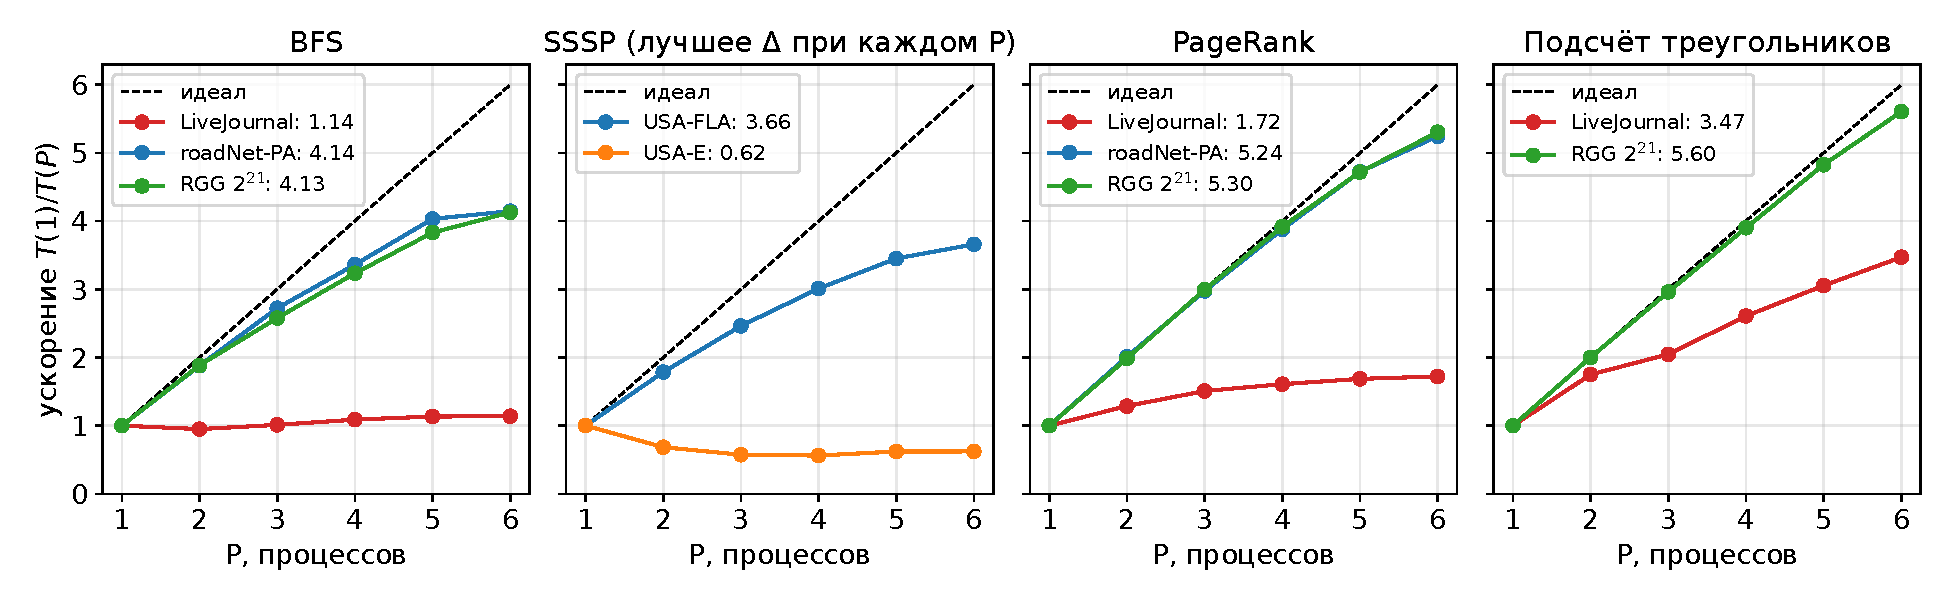
\includegraphics[width=\textwidth]{figures/speedup.pdf}
    \figcap{Ускорение $T(1)/T(P)$ при $P = 1\ldots6$ процессах, пунктир~--- идеал $S = P$,
    в легенде~--- ускорение при $P = 6$. Для SSSP при каждом $P$ взято лучшее $\Delta$}

    \begin{itemize}
        \item Графы без хабов, где у всех вершин близкая степень (дороги, RGG), ускоряются в 4--5.6 раза
        \item LiveJournal хуже всех в BFS, PageRank и TC, а SSSP на USA-E при росте $P$ замедляется
    \end{itemize}
\end{frame}

\begin{frame}
    \frametitle{BFS: время}
    \centering
    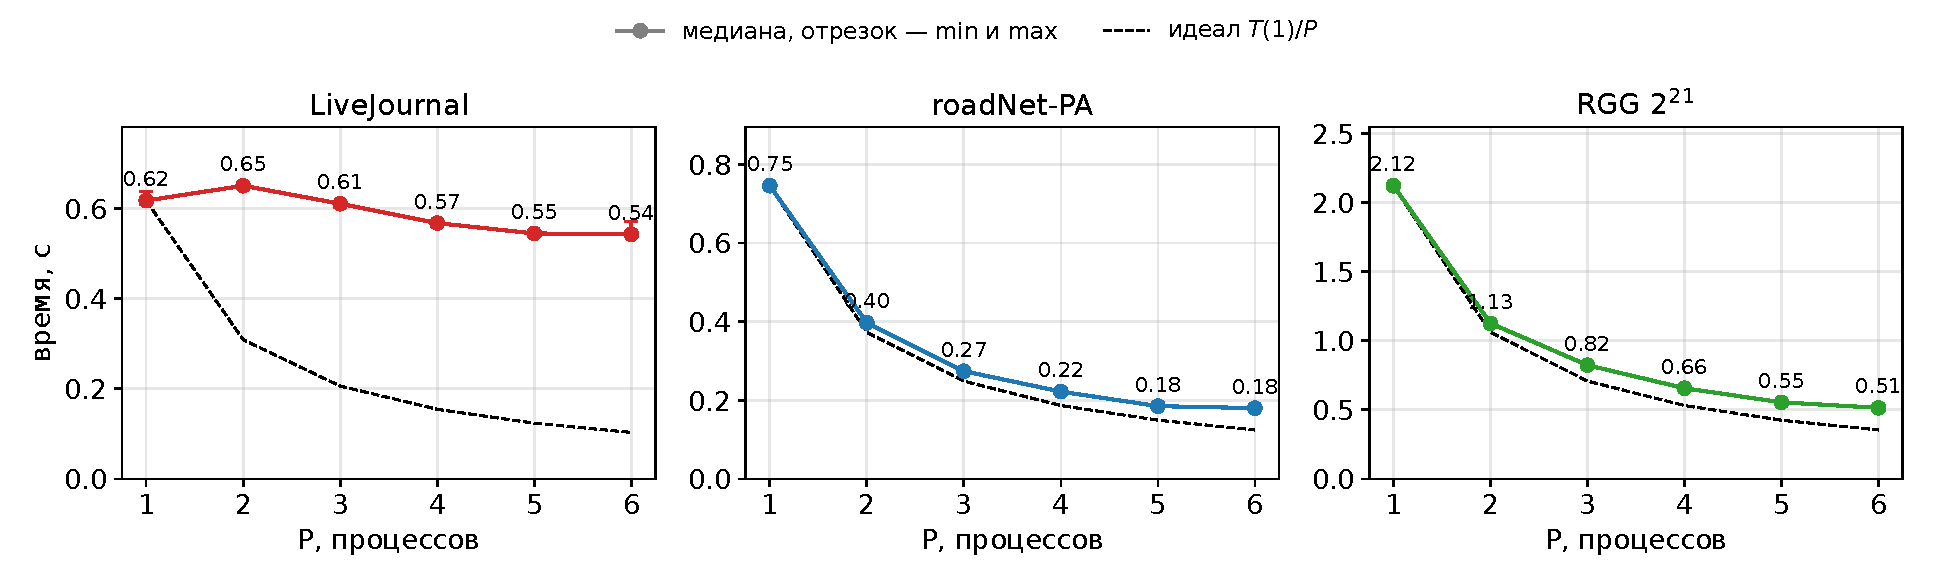
\includegraphics[width=\textwidth]{figures/bfs_time.pdf}
    \figcap{Время BFS при $P = 1\ldots6$ процессах: точка~--- медиана, отрезок~--- min и max,
    пунктир~--- идеал $T(1)/P$}

    \begin{itemize}
        \item roadNet-PA: 0.75 $\to$ 0.18~с, RGG: 2.12 $\to$ 0.51~с~--- ускорение 4.1
        \item LiveJournal: 0.62 $\to$ 0.54~с~--- почти не ускоряется
    \end{itemize}
\end{frame}

\begin{frame}
    \frametitle{BFS: время по фазам при разном $P$}
    \centering
    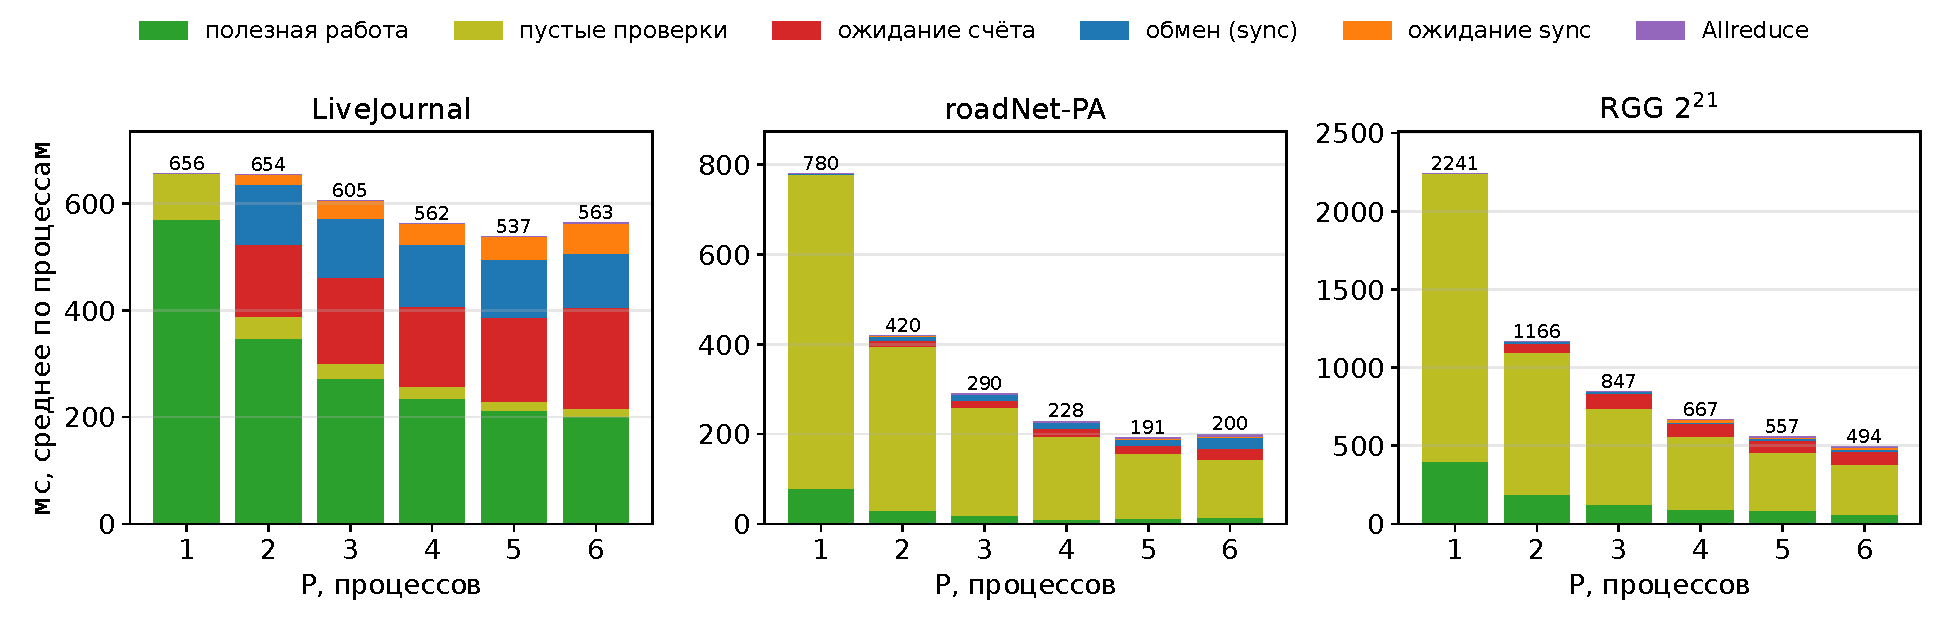
\includegraphics[width=\textwidth]{figures/bfs_phases_by_p.pdf}
    \figcap{BFS (push) при $P = 1\ldots6$: время фаз, среднее по процессам; над столбцом~--- сумма, мс.
    Данные~--- профилировщик фаз}

    \begin{itemize}
        \item roadNet-PA и RGG: при $P = 1$ почти всё~--- пустые проверки, они делятся на $P$.
              К $P = 6$ растут ожидание и обмен
        \item LiveJournal: уже при $P = 2$ ожидание и обмен съедают выигрыш от деления работы
        \item Полезная работа LiveJournal при $P = 6$~--- 200~мс, а не $571/6 \approx 95$~мс
    \end{itemize}
\end{frame}

\begin{frame}
    \frametitle{LiveJournal: промахи кэша при $P = 1$ и $P = 6$}
    \centering
    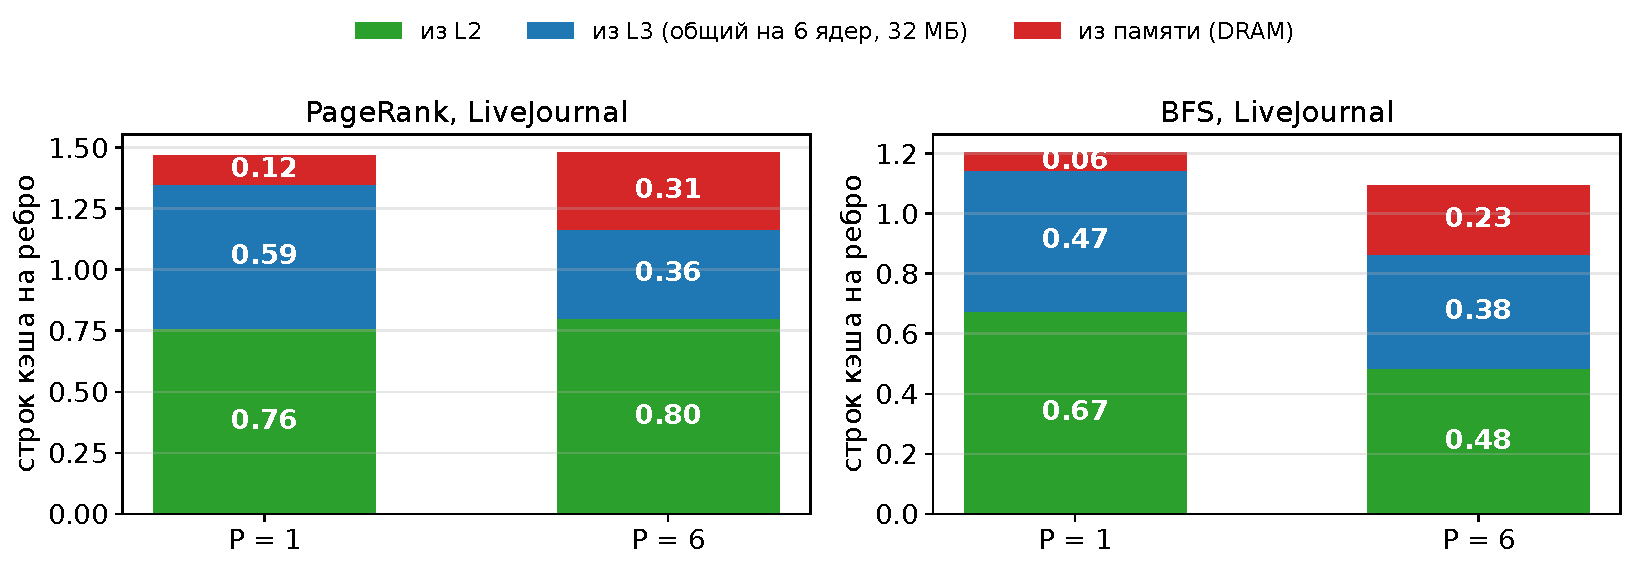
\includegraphics[width=.9\textwidth]{figures/cache_fills.pdf}
    \figcap{Откуда процессор берёт данные при промахе L1, на одно обработанное ребро: счётчики
    процессора (\texttt{perf}), сумма по процессам, один прогон без чтения графа}

    \begin{itemize}
        \item Промахов L1 на ребро столько же, но данные чаще идут из памяти, а не из L3:
              в PageRank 0.12 $\to$ 0.31 на ребро (в 2.6 раза), в BFS 0.06 $\to$ 0.23
        \item Шесть процессов делят один L3 на 32~МБ~--- рабочие данные каждого вытесняются,
              а обращение к памяти в несколько раз дороже попадания в L3
    \end{itemize}
\end{frame}

\begin{frame}
    \frametitle{BFS: на что уходит время раунда}
    \centering
    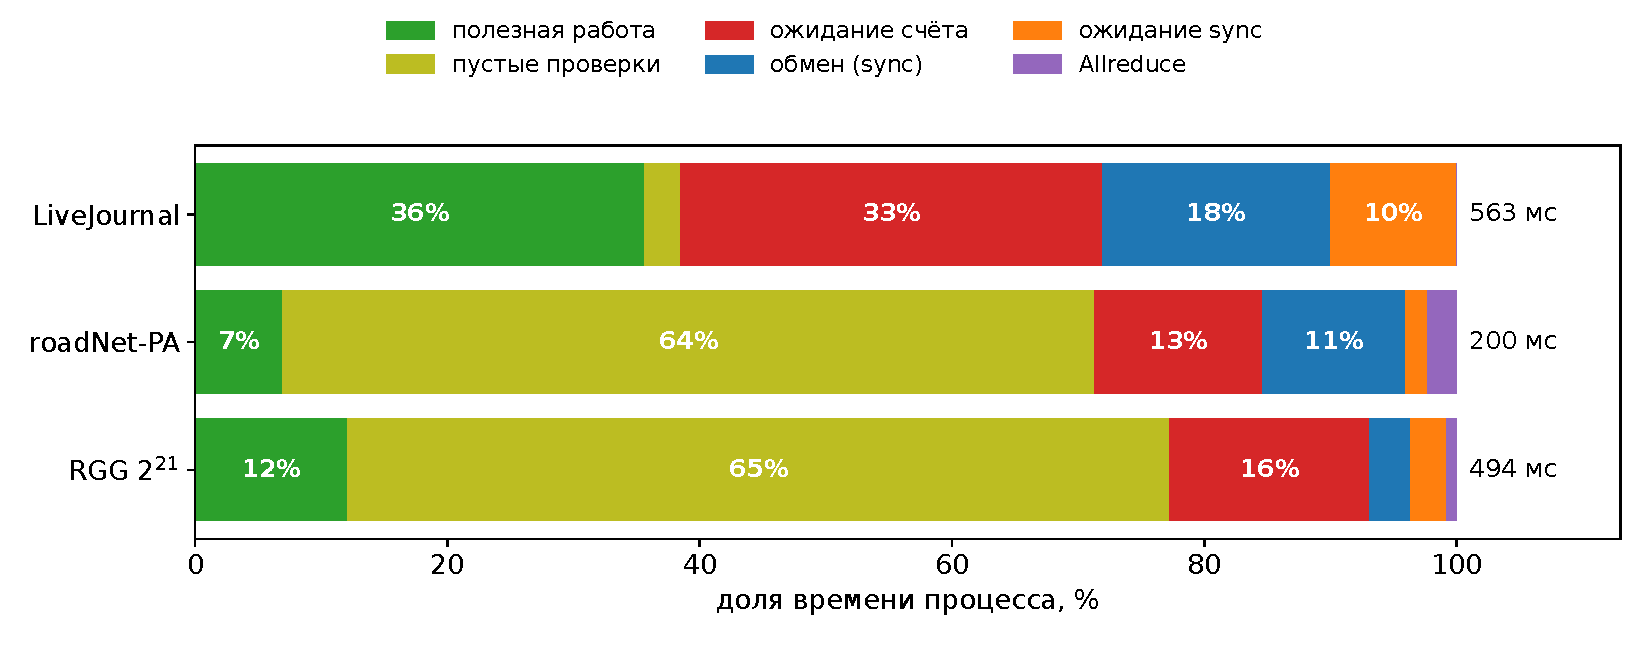
\includegraphics[width=.92\textwidth]{figures/bfs_phases.pdf}
    \figcap{BFS (push) при $P = 6$: доли фаз во времени процесса, среднее по 6 процессам,
    справа~--- время прогона. Пустые проверки~--- проход по мастерам, у которых нет работы,
    ожидание~--- процесс закончил фазу и ждёт самого медленного}

    \begin{itemize}
        \item Число раундов от $P$ не зависит: 16, 595 и 759
        \item Дороги и RGG: 64--65\% времени~--- пустые проверки: каждый раунд проходит
              \emph{всех} мастеров, а фронт~--- сотни вершин. Проход делится на $P$,
              поэтому ускорение 4.1
        \item LiveJournal: полезная работа~--- треть, ещё треть~--- ожидание, итог 1.14
    \end{itemize}
\end{frame}

\begin{frame}
    \frametitle{BFS: как работа делится между процессами}
    \centering
    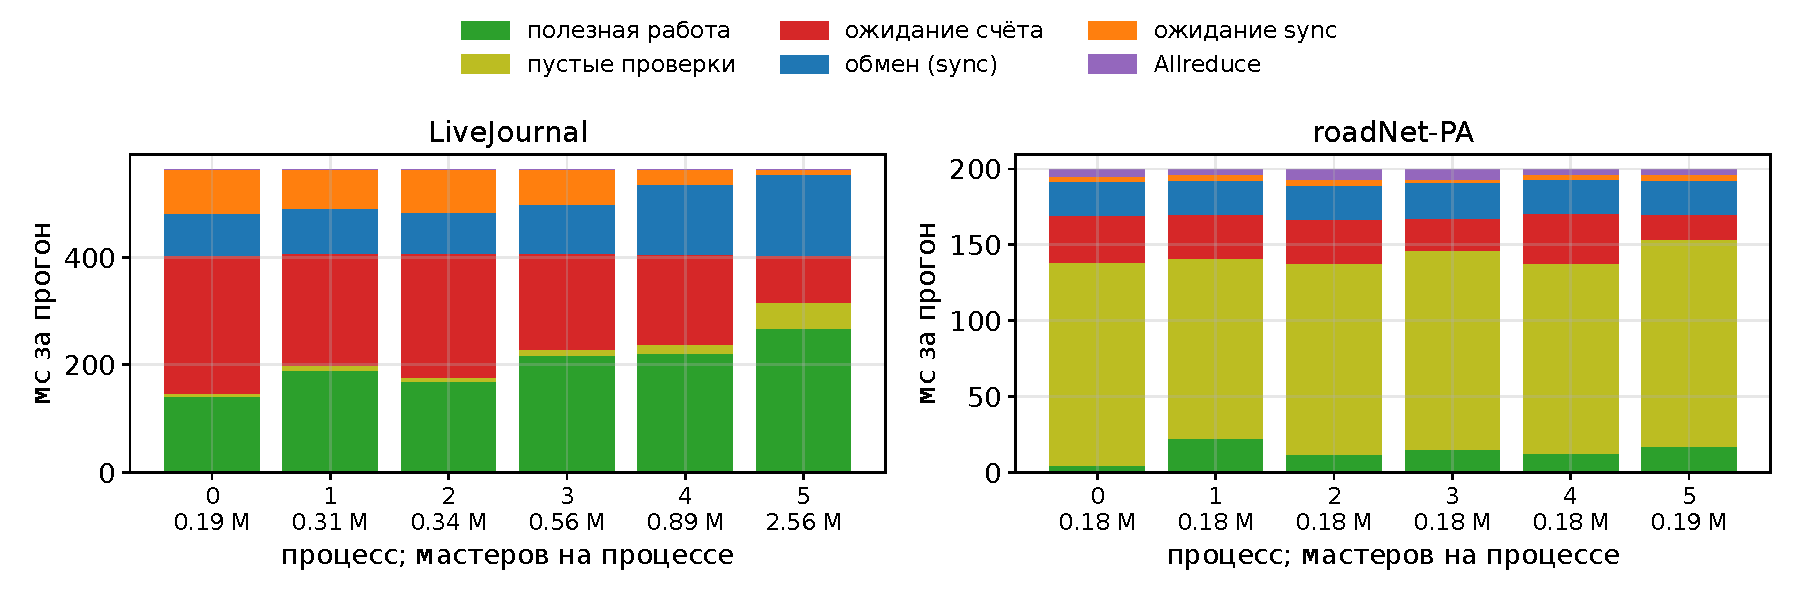
\includegraphics[width=.95\textwidth]{figures/bfs_hosts.pdf}
    \figcap{BFS при $P = 6$: время фаз на каждом процессе за прогон,
    под столбцом~--- число мастеров процесса}

    \begin{itemize}
        \item OEC делит поровну рёбра (у LiveJournal по 11.5~М), а не вершины: последнему
              процессу достаются 2.56~М вершин с малой степенью из 4.85~М
        \item LiveJournal: процесс 5 считает 268~мс, процесс 0~--- 141~мс, остальные ждут его
              (перекос $\max/\text{среднее} = 1.46$)
        \item roadNet-PA: вершины и рёбра поровну, перекос 1.08
    \end{itemize}
\end{frame}

\begin{frame}
    \frametitle{SSSP: выбор $\Delta$}
    \centering
    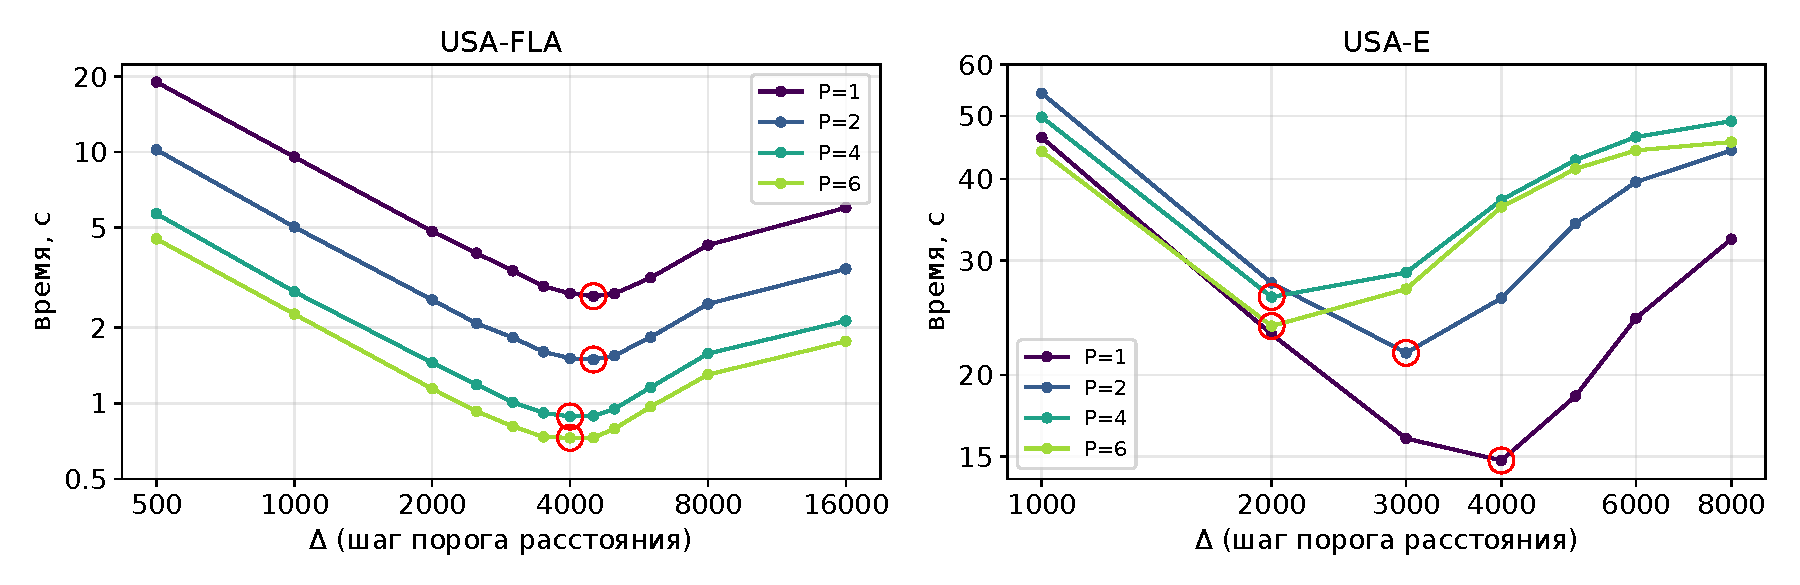
\includegraphics[width=\textwidth]{figures/sssp_delta.pdf}
    \figcap{Время SSSP от $\Delta$ при $P = 1, 2, 4, 6$ (логарифмические оси),
    красный кружок~--- лучшее $\Delta$ при данном $P$}

    \begin{itemize}
        \item За раунд обрабатываются вершины с расстоянием в полосе шириной $\Delta$:
              малое $\Delta$~--- много раундов, большое~--- лишняя работа
        \item Для сравнения по $P$ берём лучшее $\Delta$ при каждом $P$
        \item USA-FLA: лучшее $\Delta$ почти не меняется (4000--4500),
              USA-E: сдвигается с 4000 при $P = 1$ до 2000 при $P \ge 4$,
              при $\Delta = 1000$ вдвое медленнее при любом $P$
    \end{itemize}
\end{frame}

\begin{frame}
    \frametitle{SSSP: время}
    \centering
    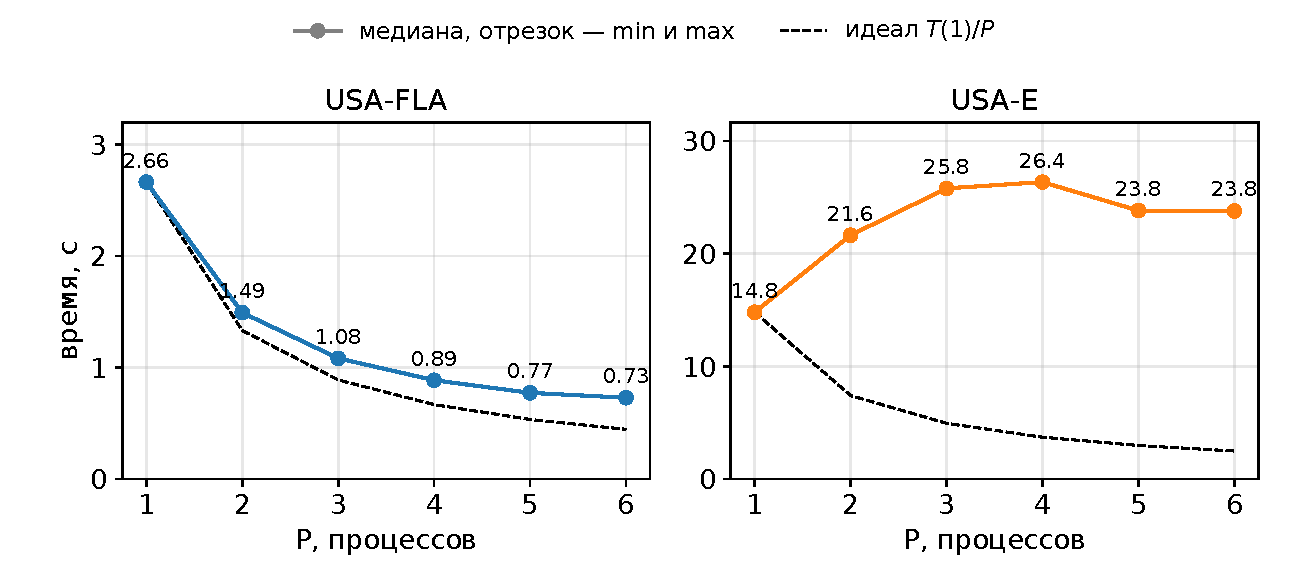
\includegraphics[width=.78\textwidth]{figures/sssp_time.pdf}
    \figcap{Время SSSP при $P = 1\ldots6$ процессах: точка~--- медиана, отрезок~--- min и max,
    пунктир~--- идеал $T(1)/P$, при каждом $P$ взято лучшее $\Delta$}

    \begin{itemize}
        \item USA-FLA: 2.66 $\to$ 0.73~с, ускорение 3.66
        \item USA-E: 14.8 $\to$ 23.8~с~--- с ростом $P$ медленнее
    \end{itemize}
\end{frame}

\begin{frame}
    \frametitle{SSSP: на что уходит время раунда}
    \centering
    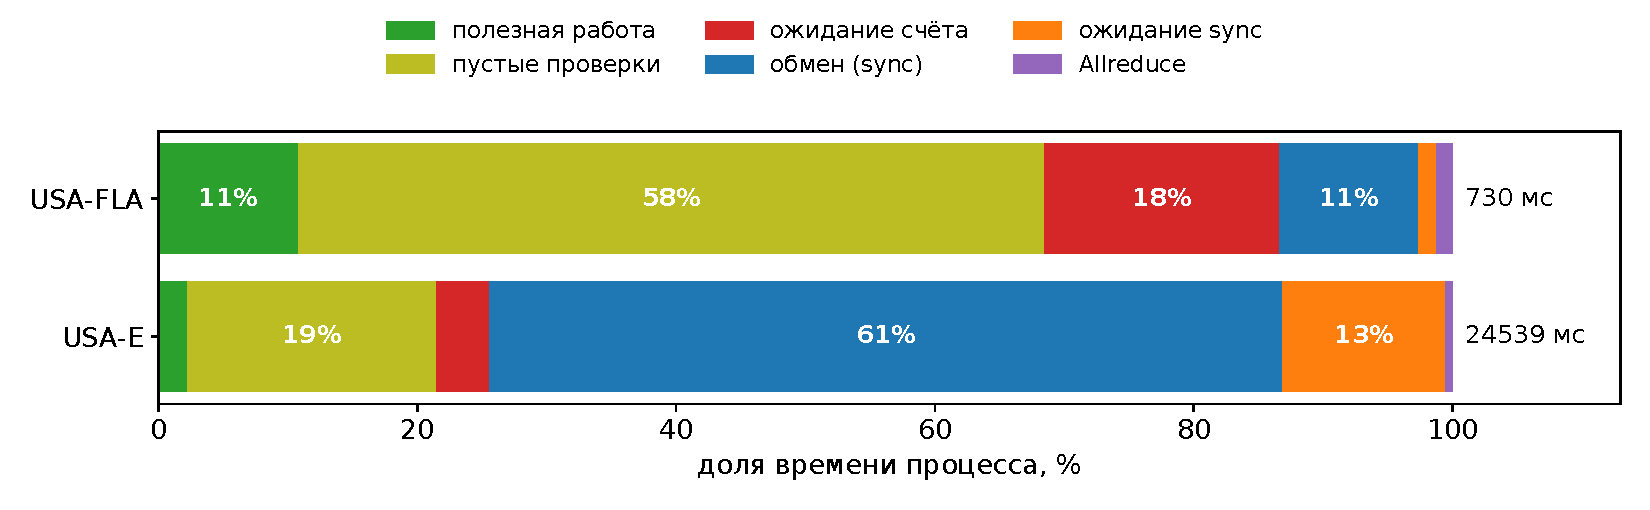
\includegraphics[width=.92\textwidth]{figures/sssp.pdf}
    \figcap{SSSP (push) при $P = 6$ и лучшем $\Delta$ (FLA~--- 4000, E~--- 2000): доли фаз во времени
    процесса, среднее по 6 процессам, справа~--- время прогона. Пустые проверки~--- проход
    по мастерам, у которых нет работы, ожидание~--- процесс закончил фазу и ждёт самого медленного}

    \begin{itemize}
        \item USA-FLA: 2120 раундов, 58\% времени~--- пустые проверки, обмен 11\%,
              ускорение 3.66
        \item USA-E: зеркал у процесса 310--880 тыс. (у FLA 1--8 тыс.), обмен~--- 61\% времени.
              Шесть процессов медленнее одного (ускорение 0.62)
    \end{itemize}
\end{frame}

\begin{frame}
    \frametitle{PageRank: время}
    \centering
    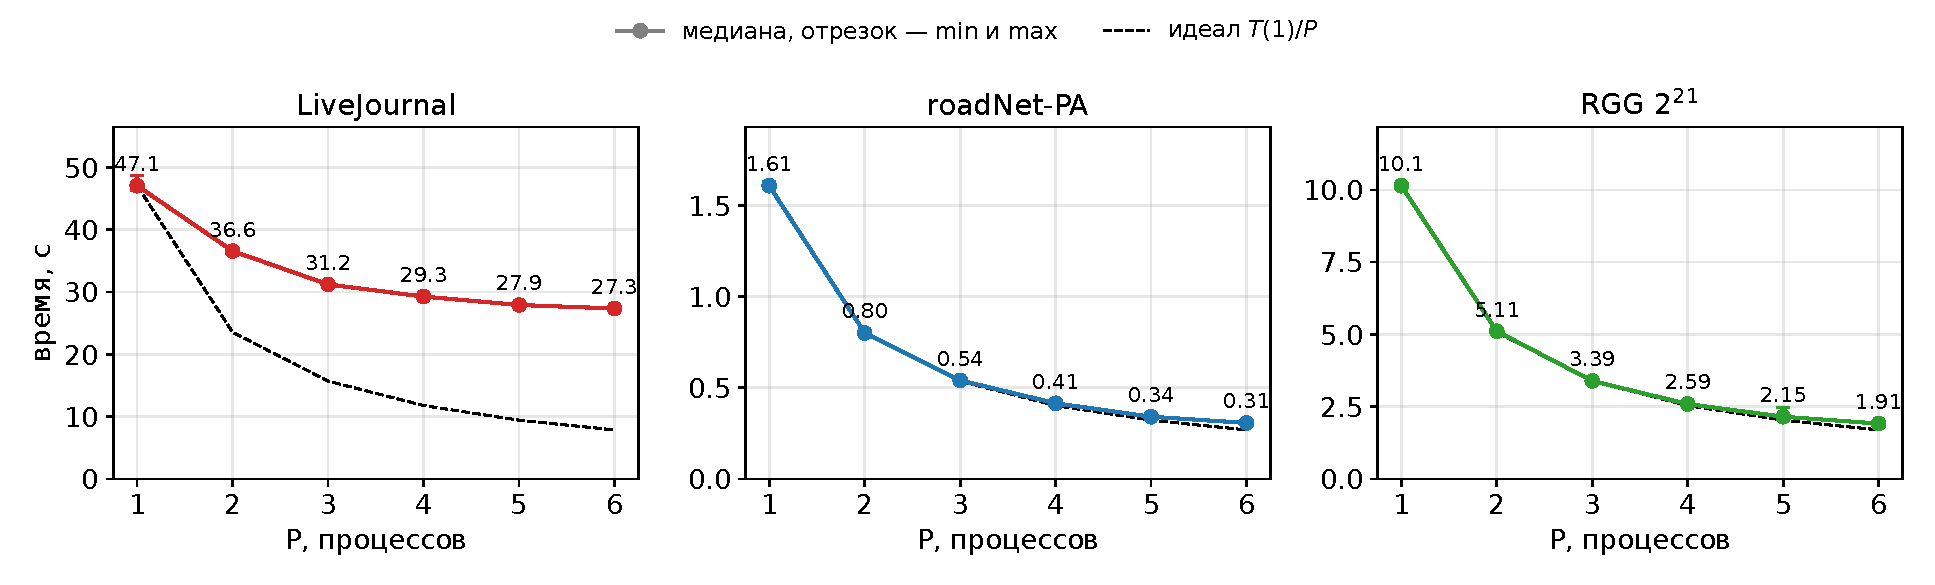
\includegraphics[width=\textwidth]{figures/pr_time.pdf}
    \figcap{Время PageRank при $P = 1\ldots6$ процессах: точка~--- медиана, отрезок~--- min и max,
    пунктир~--- идеал $T(1)/P$}

    \begin{itemize}
        \item roadNet-PA: 1.61 $\to$ 0.31~с, RGG: 10.1 $\to$ 1.91~с~--- ускорение 5.2--5.3
        \item LiveJournal: 47.1 $\to$ 27.3~с, ускорение 1.72
    \end{itemize}
\end{frame}

\begin{frame}
    \frametitle{PageRank: на что уходит время раунда}
    \centering
    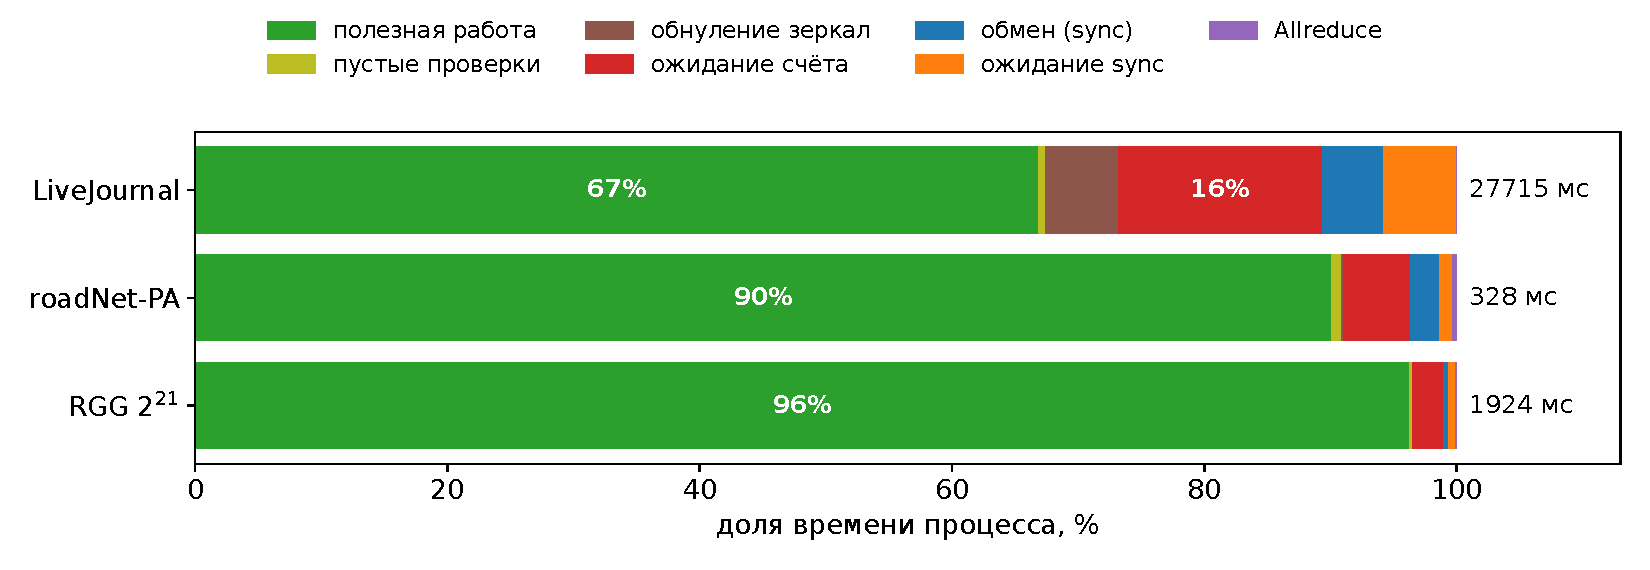
\includegraphics[width=.84\textwidth]{figures/pr.pdf}
    \figcap{PageRank (push) при $P = 6$: доли фаз во времени процесса, среднее по 6 процессам,
    справа~--- время прогона. Обнуление зеркал~--- сброс копий чужих вершин в начале каждого раунда}

    \begin{itemize}
        \item Вершины активны, пока прирост ранга больше $10^{-6}$: пустых проверок около 1\%
        \item roadNet-PA и RGG: зеркал 2--5 тыс. на процесс, полезная работа 90--96\%,
              ускорение 5.2--5.3
        \item LiveJournal: зеркал 1.2--1.8~М на процесс, обнуление и обмен~--- 11\%,
              ожидание~--- 22\%, ускорение 1.72. Рассылка дорожает из-за промахов кэша, как и в BFS
    \end{itemize}
\end{frame}

\begin{frame}
    \frametitle{Подсчёт треугольников: время}
    \centering
    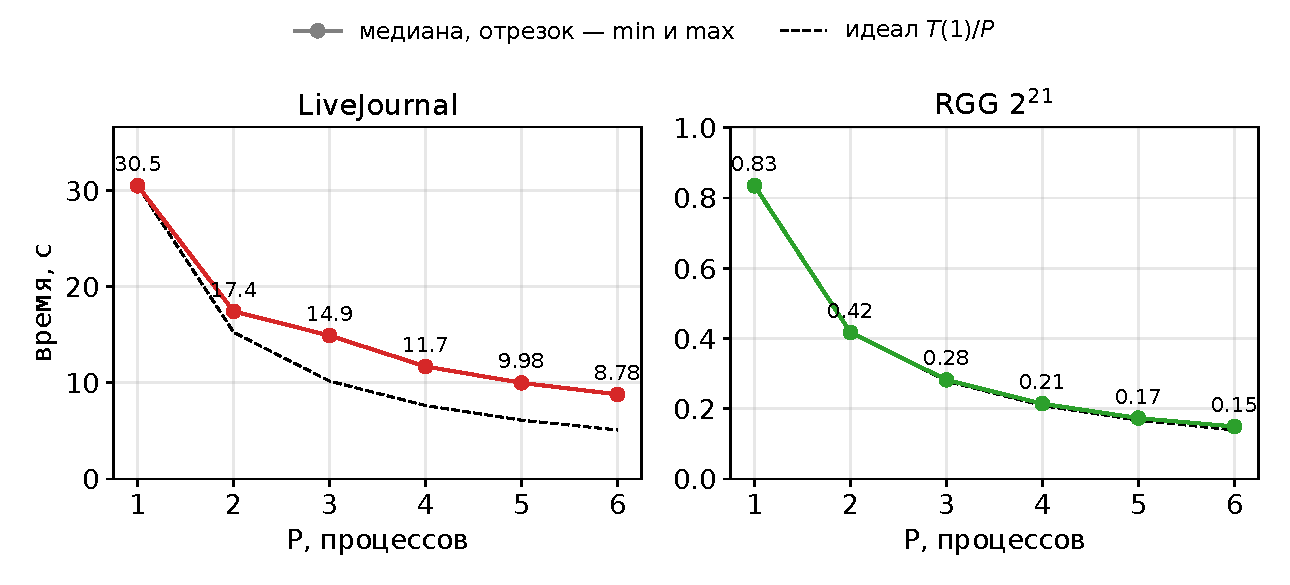
\includegraphics[width=.78\textwidth]{figures/tc_time.pdf}
    \figcap{Время подсчёта треугольников при $P = 1\ldots6$ процессах: точка~--- медиана, отрезок~--- min и max,
    пунктир~--- идеал $T(1)/P$}

    \begin{itemize}
        \item LiveJournal: 30.5 $\to$ 8.78~с, ускорение 3.47
        \item RGG: 0.83 $\to$ 0.15~с, ускорение 5.6
    \end{itemize}
\end{frame}

\begin{frame}
    \frametitle{Подсчёт треугольников}
    \centering
    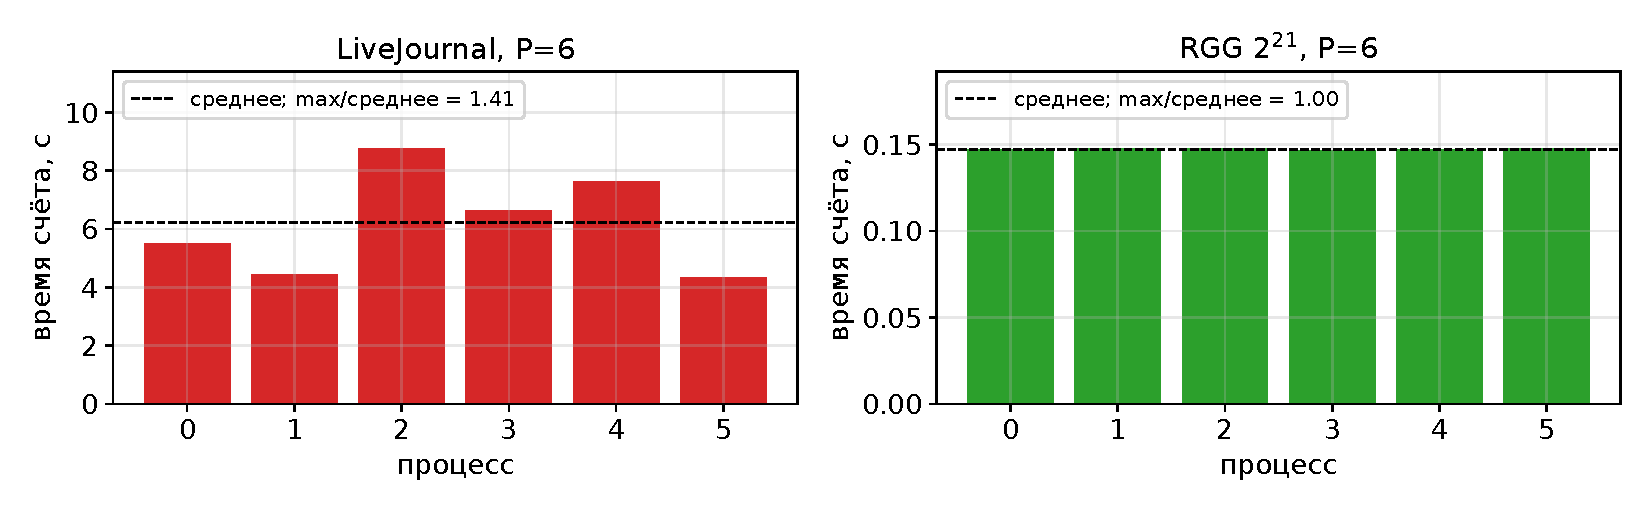
\includegraphics[width=.88\textwidth]{figures/tc_hosts.pdf}
    \figcap{Время подсчёта на каждом процессе при $P = 6$ (медиана),
    пунктир~--- среднее по процессам}

    \begin{itemize}
        \item Раундов и sync нет: один проход по мастерам и одно сложение (Allreduce)
        \item RGG: степени ровные, работа делится поровну~--- ускорение 5.6
        \item LiveJournal: работа вершины $\approx$ произведение её степени и степеней соседей, а мастера делятся
              блоками номеров~--- перекос 1.41, ускорение 3.47
    \end{itemize}
\end{frame}

\begin{frame}
    \frametitle{Результаты}
    \begin{itemize}
        \item Собран стенд: Galois, скрипты запуска и обработки, профилировщики фаз BFS,
              SSSP и PageRank (накладные расходы $< 1\%$)
        \item Измерены BFS, SSSP, PageRank и TC при $P = 1\ldots6$ на 5 графах
        \item Найдено, что ограничивает масштабируемость:
              \begin{itemize}
                  \item проходы по всем вершинам и барьер в каждом из сотен раундов (BFS на дорогах и RGG)
                  \item OEC делит поровну рёбра, а не работу: перекос на графе с хабами
                        (LiveJournal: BFS, PageRank, TC)
                  \item дорогой обмен в каждом раунде при большом RF (SSSP на USA-E: 61\% времени)
                  \item общий L3 на все процессы: при $P = 6$ обращений в память на ребро
                        в 2.6--3.8 раза больше (LiveJournal: BFS, PageRank)
              \end{itemize}
        \item Ограничение: всё мерили на одной машине, на кластере обмен дороже
    \end{itemize}
\end{frame}

\appendix

\begin{frame}
    \frametitle{Дополнительно: ширина фронта BFS}
    \centering
    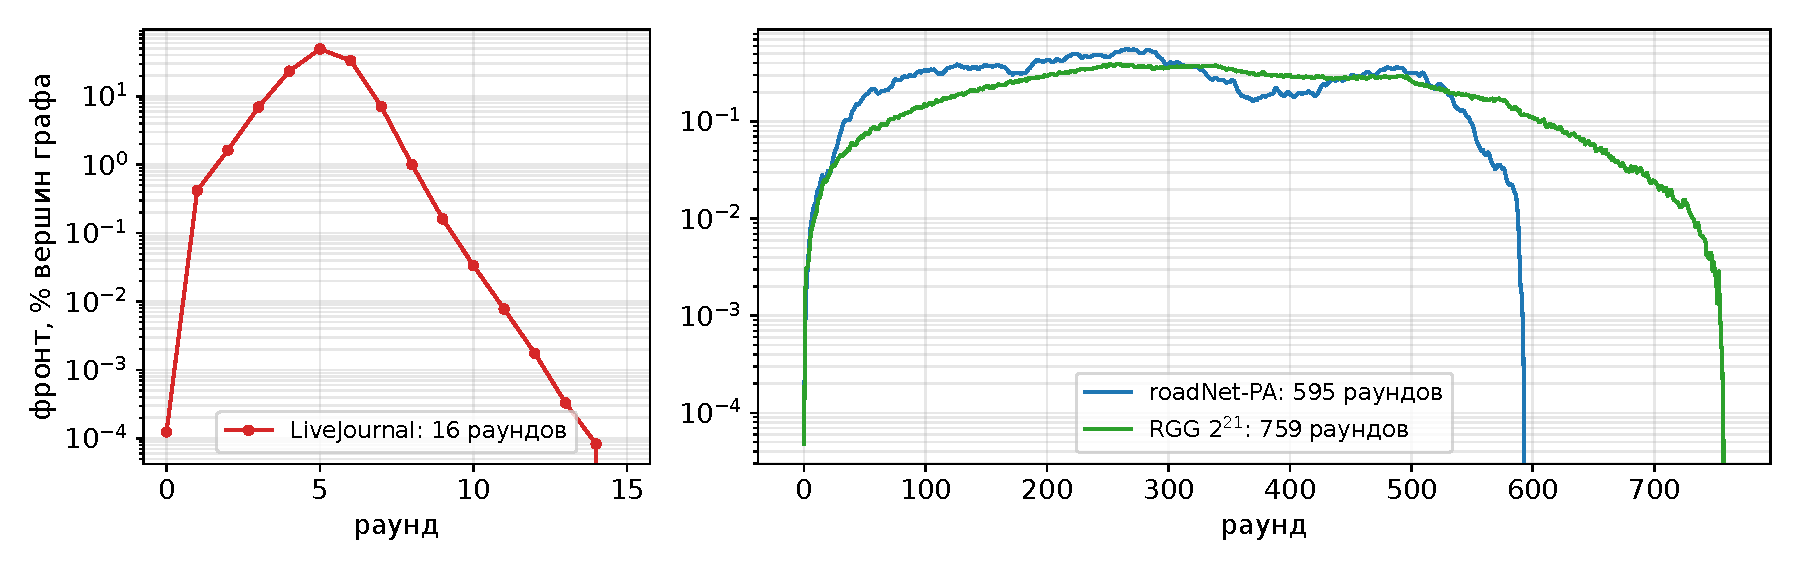
\includegraphics[width=.9\textwidth]{figures/bfs_frontier.pdf}
    \figcap{Фронт BFS~--- число вершин, которые в раунде рассылают расстояние, в процентах от всех
    вершин графа (логарифмическая ось). От $P$ не зависит. Данные~--- профилировщик при $P = 6$}

    \begin{itemize}
        \item LiveJournal: в пике активна половина графа (49\%), медиана по раундам~--- 0.42\%
        \item roadNet-PA и RGG: фронт не больше 0.6\%, медиана 0.2--0.3\%~--- остальные
              99.7\% мастеров в каждом раунде проходятся впустую
    \end{itemize}
\end{frame}

\begin{frame}
    \frametitle{Дополнительно: таймеры Galois}
    \begin{itemize}
        \item \texttt{StatTimer} копит время в микросекундах, а в статистику пишет
              целые миллисекунды и только ненулевой итог
        \item \texttt{Timer\_N} создаётся один раз на прогон $N$ вокруг основного цикла
              алгоритма~--- точность $\pm 1$~мс
        \item Таймеры счёта (\texttt{do\_all}) и sync создаются заново \emph{в каждом раунде}:
              раунд короче 1~мс даёт 0 и не записывается. SSSP на FLA, $\Delta = 500$, $P = 6$:
              счёт \enquote{14~мс} за весь прогон
        \item Поэтому фазы раунда меряет свой профилировщик (\texttt{steady\_clock}, мкс),
              ожидание выводится из меток времени: у процессов на одной машине общие часы
    \end{itemize}
\end{frame}

\begin{frame}
    \frametitle{Дополнительно: RF по графам}
    \begin{columns}[c]
        \begin{column}{.48\textwidth}
            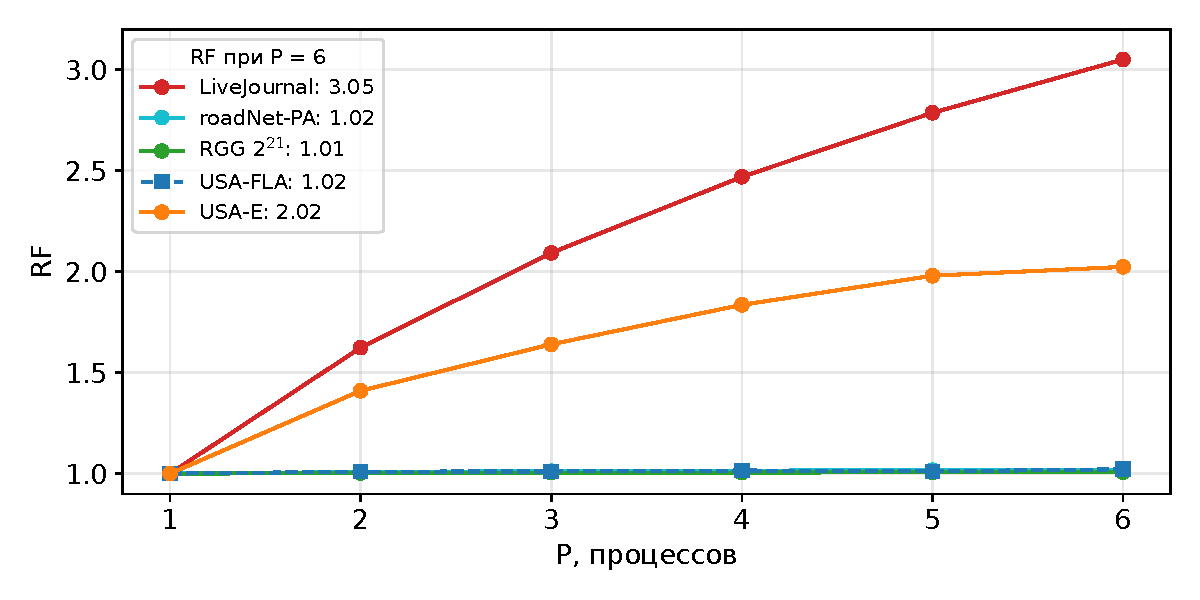
\includegraphics[width=\textwidth]{figures/rf.pdf}
        \end{column}
        \begin{column}{.52\textwidth}
            \centering
            \footnotesize
            \begin{tabular}{lrrrrr}
                \toprule
                Граф & $P{=}2$ & 3 & 4 & 5 & 6 \\
                \midrule
                LiveJournal & 1.62 & 2.09 & 2.47 & 2.79 & 3.05 \\
                USA-E       & 1.41 & 1.64 & 1.84 & 1.98 & 2.02 \\
                USA-FLA     & 1.01 & 1.01 & 1.02 & 1.01 & 1.02 \\
                roadNet-PA  & 1.01 & 1.01 & 1.01 & 1.02 & 1.02 \\
                RGG $2^{21}$ & 1.00 & 1.00 & 1.01 & 1.01 & 1.01 \\
                \bottomrule
            \end{tabular}
        \end{column}
    \end{columns}
    \figcap{RF~--- среднее число копий вершины (мастер и зеркала) по всем процессам
    при разбиении OEC, $P = 1\ldots6$; при $P = 1$ RF $= 1$}

    \begin{itemize}
        \item LiveJournal: у хабов соседи на всех процессах, RF растёт до 3.05
        \item USA-E: номера вершин плохо ложатся на блоки, RF до 2.02
        \item Дороги FLA, roadNet-PA и RGG: соседи почти всегда в том же блоке номеров, RF $\le 1.02$
    \end{itemize}
\end{frame}

\end{document}
